The distribution $P(\B \sigma)$ of all possible peptides $\B \sigma$ within an organism is highly undersampled for even moderate length peptides. Still we can pursue a statistical approach and assign a probability to each peptide that measures how likely such a peptide is on average given the underlying proteome statistics.

We constrain some statistical observables $\langle f_\mu(\boldsymbol \sigma)\rangle$ to be equal to their empirical values $\bar{f_\mu}$, while otherwise keeping the probability distribution as random as possible. In mathematical terms this means that we are looking for the probability distribution that maximizizes the Shannon entropy
\begin{equation}
    S[P(\B \sigma)] = - \sum_{\B \sigma} P(\B \sigma) \log P(\B \sigma),
\end{equation}
subject to a normalization constraint and a constraint
\begin{equation}
    \langle f_\mu(\boldsymbol \sigma)\rangle = \sum_{\boldsymbol \sigma} P(\boldsymbol \sigma) f_\mu(\boldsymbol \sigma) = \bar{f_\mu},
\end{equation}
for each observable.
The optimization with respect to the normalization constraint can be performed analytically, which yields a Boltzmann distribution of the following form
\begin{equation}
    P(\boldsymbol \sigma) = \frac{1}{Z} \exp\left[ -E(\B \sigma) \right].
\end{equation}
with 
\begin{equation}
 E(\B \sigma) = \sum_{\mu=1}^K \lambda_\mu f_\mu(\boldsymbol \sigma)
\end{equation}
and 
\begin{equation}
    Z = \sum_{\B \sigma} \exp \left[ - E(\B \sigma) \right]
\end{equation}
    is a normalization factor, called the partition function in statistical mechanics.
We fit the model parameters using Boltzmann machine learning. To do so we estimate $\langle f_\mu(\B \sigma)\rangle$ using Monte Carlo methods for given model parameters. The parameters are then updated by gradient ascent,
\begin{equation}
    \lambda_\mu^{t+1} = \lambda_\mu^t + \epsilon_\mu^t \left(\langle f_\mu \rangle  - \bar{f_\mu}\right),
\end{equation}
where $\epsilon_\mu^t$ represents a learning rate (which generally can be coordinate dependent and time-varying).


\begin{figure*}
    \includegraphics[width=\textwidth]{maxent_freqs}
    \caption{Connected correlation functions of a maximum entropy model based on 1 and 2-point frequencies ressemble those of the training test set (upper row) within the training and test set error (lower row). Color indicates local density in regions with overplotting.
    \label{figmaxent_freqs}
    }
\end{figure*}

A common choice is to constrain the one and two-point frequencies
\begin{align}
    f_i^\alpha(\B \sigma) &= \sigma_i^\alpha, \\
    f_{ij}^{\alpha\beta}(\B \sigma) &= \sigma_i^\alpha \sigma_j^\beta,
\end{align}
where $\sigma_i^\alpha = 1$ if the amino acid at site i is of type $\alpha$ and zero otherwise.
This leads to a maximum entropy probability distribution that takes the form of a disordered Potts model,
\begin{equation}
    E(\boldsymbol \sigma) = - \sum_{i=1}^L \sum_{\alpha = 1}^{20} h_i^\alpha \sigma_i^\alpha - \sum_{i<j}^L \sum_{\alpha,\beta = 1}^{20} J_{ij}^{\alpha \beta}  \sigma_i^\alpha \sigma_j^\beta.
\end{equation}
The fitted model reproduces the 1- and 2-point connected correlations indicating fit convergence (Fig.~\ref{figmaxent_freqs}A,B). The model predicted connected third order correlations follow a similar trend between model and data, but are generally underestimated (Fig.~\ref{figmaxent_freqs}C).


\begin{figure*}
    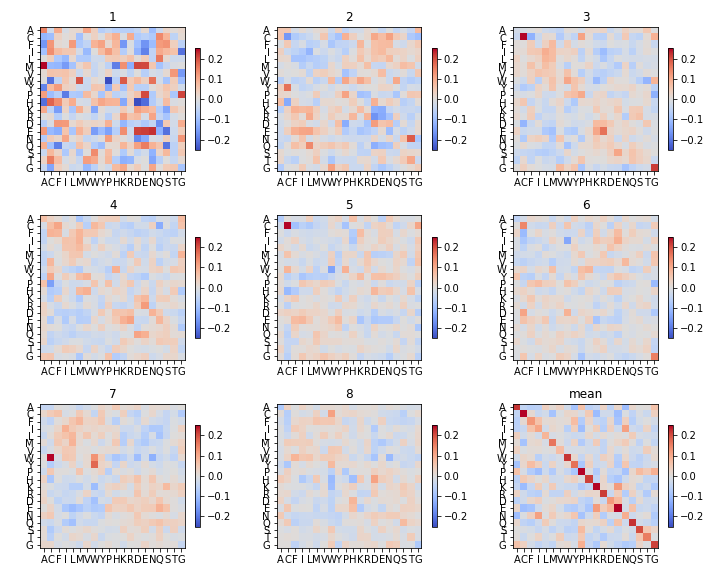
\includegraphics[width=\textwidth]{Jij_vs_dist}
    \caption{Mean coupling and deviations from mean coupling at a given distance. 
    \label{figJij_vs_dist}
    }
\end{figure*}


\begin{figure*}
    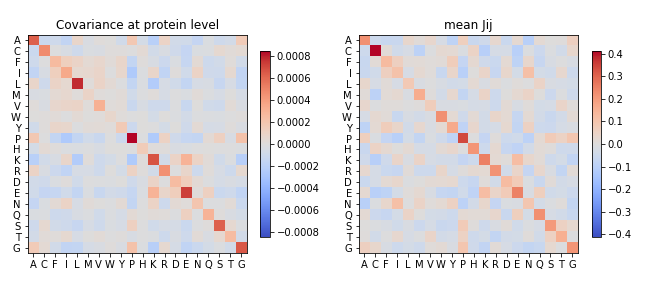
\includegraphics[width=\textwidth]{meanJij_aacovariance}
    \caption{Mean coupling matrix and covariance matrix between amino acid composition at protein level.
    \label{figJij_aacovariance}
    }
\end{figure*}


\begin{figure*}
    \includegraphics[width=\textwidth]{maxent_freqs_global}
    \caption{Correlation between compositional Maxent model and test set (upper row) and training and test set (lower row) for the first three connected correlation functions.
    \label{figmaxent_freqs_global}
    }
\end{figure*}

Given that many biases are compositional in nature we can also consider a simpler model that only involves a global constraint on the covariation of the total count of amino acids of different types:
\begin{align}
    n^\alpha(\B \sigma) &= \sum_i \sigma_i^\alpha, \\
    n^{\alpha\beta}(\B \sigma) &= n^\alpha(\B \sigma) n^\beta(\B\sigma) = \left(\sum_{i=1}^L \sigma_i^\alpha\right) \left(\sum_{j=1}^L \sigma_j^\beta\right).
\end{align}
This leads to a maximum entropy probability distribution that takes the form
\begin{equation}
    E(\boldsymbol \sigma) = - \sum_{\alpha=1}^{20} h^\alpha n^\alpha -  \sum_{\alpha,\beta = 1}^{20} J^{\alpha \beta} n^\alpha n^\beta,
\end{equation}
i.e. a model that only involves global couplings between amino acids independent of their distance.
A model with such global couplings captures a large fraction of 2-point correlations (Fig.~\ref{figmaxent_freqs_global}B), in line with the expectation that many of the constraints on amino acid covariation reflect compositional differences between different classes of proteins.


\begin{figure*}
    \includegraphics{dos}
    \caption{Density of states with respect to the 2-point model energy function for kmers from the test set and model-drawn kmers.
    \label{figdos}
    }
\end{figure*}

\begin{figure}
    \includegraphics[width=\columnwidth]{hammingdist}
    \caption{Distribution of Hamming distances between random pairs of sequences from the model and the test set normalized by expectation from comparison of training and test set sequences. The observed dip at small distances reveals further structure not captured by any of the models.
    \label{fighammingdist}
    }
\end{figure}



Once we have fitted the model parameters we can calculate the entropy of the distribution $P(\B \sigma)$. To do so we use the identity
\begin{align}
    S &= - \sum_{\B \sigma}  P(\B \sigma) \log P(\B \sigma),  \\
      &= \langle E(\B \sigma) \rangle - F, \quad F = - \log Z.
\end{align}
The mean energy can be calculated directly from Monte Carlo samples. To calculate the free energy we use thermodynamic integration as follows \cite{Marchi2019b}: We express the energy with respect to a reference energy $E_{ref}(\B \sigma)$ as $E(\B \sigma) = E_{ref}(\B \sigma) + \Delta E(\B\sigma)$, where the reference energy is choosen such that $F_{ref}$ can be calculated analytically. We define the perturbed energy function
\begin{equation}
    E_\alpha(\B \sigma) = E_{ref}(\B \sigma) + \alpha \Delta E(\B\sigma),
\end{equation}
which scales the contribution of the energy beyond the reference model.
To obtain the free energy we use the identity
\begin{equation}
    F(1) = F_{ref} + \int_0^1 \ud \alpha F'(\alpha).
\end{equation}
Note that
\begin{equation}
    F'(\alpha) = - \langle \Delta E(\B \sigma) \rangle_{\alpha},
\end{equation}
which allows us to approximate the integrand by Monte Carlo simulations. We numerically evaluate $F'(\alpha)$ for evenly spaced $\alpha \in [0, 1]$ and calculate the integral by Simpson's rule. Calculating the entropy in this way allows us to determine the reduction in the effective diversity in sequences implied by including different constraints (Fig.~\ref{figdiversity_reduction}). 

\begin{figure}
    \includegraphics{diversity_reduction}
    \caption{Effective diversity of modelled distributions of 9-mers including different constraints.
    \label{figdiversity_reduction}
    }
\end{figure}





